\documentclass[8pt]{beamer}

\usepackage[utf8]{inputenc}
\usepackage[T1]{fontenc}
\usepackage{lmodern}
\usepackage{amsmath}
\usepackage[normalem]{ulem}
\usepackage{tikz}
\usepackage{hyperref}
\usepackage{listings}

\definecolor{links}{HTML}{2A1B81}
\hypersetup{colorlinks,linkcolor=,urlcolor=links}

\lstset{
  basicstyle=\footnotesize\ttfamily,
  numbers=left,
  numbersep=-2em,
  numberstyle=\color{gray}
}

\usetikzlibrary{shapes,arrows,automata}

\tikzset{
  vertex/.style={
    rectangle,
    rounded corners,
    draw=black, thick,
    text centered
  },
}

\mode<beamer>
{
  \usetheme{Frankfurt}
  \useoutertheme{miniframes}
  \setbeamercovered{transparent}
}

\subject{Talks}

\AtBeginSection[]
{
  \begin{frame}<beamer>{}
    \tableofcontents[currentsection]
  \end{frame}
}

\title[LLVM]{LLVM: Low Level Virtual Machine\\An introduction to compiler infrastructure}
\author[Krystian Bacławski]{\href{mailto:cahirwpz@cs.uni.wroc.pl}{Krystian Bacławski}}
\institute{Computer Science Department\\University of Wrocław}
\date{\today}

\begin{document}

\begin{frame}
\titlepage
\end{frame}

\section[Introduction]{What is LLVM?}
\subsection*{Introduction}

\begin{frame}[fragile]{Introduction}
  \begin{block}{LLVM is a software framework for building compilers.}
    \begin{itemize}
      \item Well-defined intermediate code representation (aka LLVM IR -- \verb+.ll+ files).
      \item Binary representation of LLVM IR (\verb+.bc+ files).
      \item Code generators for many hardware architectures (\verb+x86+,
        \verb+mips+, \verb+arm+, \verb+sparc+, \verb+ppc+).
      \item Low-level optimizations (triggered during code generation phase).
      \item Just-in-Time compilation and execution subsystem.
      \item IR code transformations and optimizations (for use by an optimizing compiler).
      \item Linkable and executable file handling (\verb+ELF+, \verb+MachO+, \verb+COFF+).
      \item Tools like assembler, disassembler, optimizer and so on.
    \end{itemize}
  \end{block}

  \begin{block}{What LLVM is not?}
    \begin{description}
      \item[\sout{a compiler}] though one can use it to implement a mid-bottom part of a compiler.
      \item[\sout{a library}] set of libraries, tools and a run-time environment.
    \end{description}
  \end{block}
\end{frame}

\begin{frame}[fragile]{Applications}
  \begin{block}{Research platform:}
    \begin{itemize}
      \item Experiments with low-level and mid-level optimizations.
      \item Code profiling and instrumentation.
      \item ISA (instruction set architecture) design.
      \item Compilers for domain specific languages.
    \end{itemize}
  \end{block}

  \begin{exampleblock}{Notable LLVM uses:}
    \begin{itemize}
      \item Clang (C, C++, ObjC and ObjC++ front-end)
      \item Compilers: Haskell, NVIDIA CUDA, Erlang HiPE,
      \item Interpreters: PyPy, Mono, IcedTea, ClamAV,
      \item GPGPU: OpenCL, Apple's OpenGL,
      \item LLDB -- GNU Debugger competitor,
      \item ASAN and TSAN -- code instrumentation for debugging purposes,
      \item and so on\ldots (\href{http://llvm.org/Users.html}{LLVM Users})
    \end{itemize}
  \end{exampleblock}
\end{frame}

\begin{frame}[fragile]{Competition}
  \begin{block}{LLVM together with Clang and LLDB tries to compete with GNU Toolchain}
    \begin{itemize}
      \item object and archive manipulation (\verb+ar+, \verb+ranlib+,
        \verb+nm+, \verb+objdump+, \verb+readobj+)
      \item profiler (\verb+prof+, \verb+cov+)
      \item compiler, assembler and linker (\verb+clang+)
      \item debugger (\verb+lldb+)
    \end{itemize}
  \end{block}

  \begin{alertblock}{Especially Clang is worth a look!}
    \begin{itemize}
      \item It offers easy to understand diagnostic messages:
        \begin{itemize}
          \item especially for C++ templates and namespaces,
          \item more meaningful warnings!
        \end{itemize}
      \item \ldots superior (memory and time) efficiency compared to GCC,
      \item \ldots and a fast C / C++ parser library for:
        \begin{itemize}
          \item high-level optimizations,
          \item static analysis,
          \item program transformations.
        \end{itemize}
      \item Is an area of interesting (and practical) research:
        \begin{itemize}
          \item modules for C language,
          \item thread-safety annotation checking.
        \end{itemize}
    \end{itemize}
  \end{alertblock}
\end{frame}

\section[Overview]{Framework overview}
\subsection*{Program structure}

\begin{frame}{Stream of instructions}
  \begin{block}{How CPU perceives a program?}
    \begin{itemize}
      \item A stream of instruction and bulk of data.
      \item A stream is composed of mix of arithmetic and control flow instructions.
      \item An OS knows the start execution of a stream and gives a method to
        finish it.
      \item CPU is not concerned with instruction stream structure (functions,
        modules, etc.)
    \end{itemize}
  \end{block}

  \begin{block}{Control flow graph}
    \begin{itemize}
      \item Let's organize instructions into a directed graph.
      \item Each node stores a list of (arithmetic) instructions \ldots
      \item and finishes with exactly one PC-modifying instruction.
      \item Input degree of a node is of arbitrary order.
      \item Output degree is one or two (jump / call / return or conditional branch).
    \end{itemize}
  \end{block}
\end{frame}

\begin{frame}{Need for Application Binary Interface}
  \begin{block}{How symbols are represented? (name mangling)}
    \begin{itemize}
      \item A mapping from identifier and object's type into a link-time symbol.
      \item Do we need to encode function's signature into a symbol (due to overloading)?
      \item Any attributes associated with a symbol (visibility, linking, optimization)?
    \end{itemize}
  \end{block}
    
  \begin{block}{How to call a function? (calling convention)}
    \begin{itemize}
      \item Where to put arguments (stack or registers)?
      \item Where the result is available?
      \item How to create activation record?
      \item Which registers need to be saved and restored?
    \end{itemize}
  \end{block}

  \begin{block}{How is data organized in memory?}
    \begin{itemize}
      \item Which bit is MSB and LSB?
      \item Big-endian or little-endian?
      \item Alignment requirements for words?
      \item Size of machine data types (integer, float, etc.)?
    \end{itemize}
  \end{block}
\end{frame}

\subsection*{LLVM intermediate language}

\begin{frame}[fragile]{Virtual machine model}
  \begin{block}{Implemented model:}
    \begin{itemize}
      \item Register based machine -- infinite number of virtual registers.
      \item Implicit stack -- no stack management else than variable placement.
      \item Instruction stream in SSA (static single assignment) form.
      \item Strongly typed machine:
        \begin{itemize}
          \item explicit coercions between numeric machine types,
          \item typed pointers!
        \end{itemize}
      \item RISC-like load-store approach to memory access.
      \item Compound (structures) and aggregate types (vectors).
      \item Heavily influenced by \verb+C+ language but versatile enough.
    \end{itemize}
  \end{block}
  
  \begin{block}{Some interesting extra features:}
    \begin{itemize}
      \item Language agnostic exception handling (incl. DWARF2 stack unwinding).
      \item Support for accurate garbage collection.
      \item Atomic memory access for concurrent programming.
    \end{itemize}
  \end{block}
\end{frame}

\begin{frame}[fragile]{SSA form}
  \begin{figure}[!h]
    \centering
    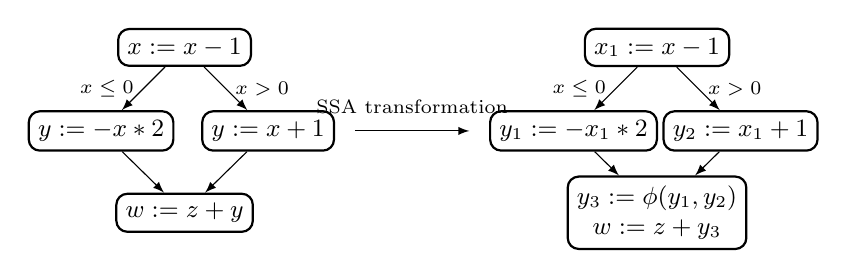
\begin{tikzpicture}[auto,node distance=1.5cm,font=\small]
      \begin{scope}
        \node[vertex] (a) {$x := x - 1$};
        \node[vertex, below left of=a] (b) {$y := -x * 2$};
        \node[vertex, below right of=a] (c) {$y := x + 1$};
        \node[vertex, below of=a,yshift=-0.6cm] (d) {$w := z + y$};
        \path[->,font=\scriptsize,>=latex]
        (a) edge node[left]{$x \leq 0$} (b)
        (a) edge node[right]{$x > 0$} (c)
        (b) edge (d)
        (c) edge (d);
      \end{scope}

      \begin{scope}[xshift=6cm]
        \node[vertex] (a') {$x_1 := x - 1$};
        \node[vertex, below left of=a'] (b') {$y_1 := -x_1 * 2$};
        \node[vertex, below right of=a'] (c') {$y_2 := x_1 + 1$};
        \node[vertex, below of=a',yshift=-0.6cm,align=center]
        (d') {$y_3 := \phi(y_1,y_2)$ \\ $w := z + y_3$};
        \path[->,font=\scriptsize,>=latex]
        (a') edge node[left]{$x \leq 0$} (b')
        (a') edge node[right]{$x > 0$} (c')
        (b') edge (d')
        (c') edge (d');
      \end{scope}

      \draw [->,>=latex,shorten >=2.5mm,shorten <=2.5mm] (c) -- (b')
      node [above=1mm,font=\scriptsize,midway,text centered] {SSA transformation};
    \end{tikzpicture}
    \caption{Example of SSA transformation for simple \texttt{if-then-else} statement.}
  \end{figure}

  \begin{block}{\textit{Static Single Assignment} form properties}
    \begin{itemize}
      \item Variables, once assigned, cannot be changed.
      \item $\phi(\ldots)$ operator for expressing imperative constructs like
        \verb+if-then-else+ or \verb+while+.
      \item Thanks to immutability better properties for code analysis
        algorithms.
      \item Some optimizations are available almost for free (eg. dead code
        elimination).
      \item Well known algorithm for SSA transformation (dominance frontiers).
    \end{itemize}
  \end{block}

\end{frame}

\begin{frame}[fragile]{Basic instructions}
  \begin{block}{}
    \begin{itemize}
      \item Arithmetic instructions:
        \begin{itemize}
          \item integer: \verb+add+, \verb+sub+, \verb+mul+, \verb+udiv+,
            \verb+sdiv+, \verb+urem+, \verb+srem+, \verb+icmp+
          \item floating-point: \verb+fadd+, \verb+fsub+, \verb+fmul+, \verb+fdiv+,
            \verb+frem+, \verb+fcmp+
        \end{itemize}

      \item Bitwise instructions:
        \begin{itemize}
          \item bit-shift: \verb+shl+, \verb+lshr+, \verb+ashr+
          \item boolean: \verb+and+, \verb+or+, \verb+xor+
        \end{itemize}

      \item Control flow instructions:
        \begin{itemize}
          \item function calls: \verb+invoke+, \verb+call+, \verb+ret+
          \item jumping: \verb+br+, \verb+switch+, \verb+indirectbr+
          \item other: \verb+phi+, \verb+select+
        \end{itemize}

      \item Memory access instructions:
        \begin{itemize}
          \item stack space allocation: \verb+alloca+
          \item generic accessors: \verb+load+, \verb+store+
        \end{itemize}

      \item Compound data access instructions:
        \begin{itemize}
          \item vectors: \verb+extractelement+, \verb+insertelement+, \verb+shufflevector+
          \item aggregates: \verb+extractvalue+, \verb+insertvalue+
          \item other: \verb+getelementptr+
        \end{itemize}

      \item Data conversion instructions:
        \begin{itemize}
          \item integer: \verb+trunc+, \verb+zext+ \verb+sext+
          \item floating-point: \verb+fptrunc+, \verb+fpext+, \verb+fptoui+,
            \verb+fptosi+, \verb+uitofp+, \verb+sitofp+,
          \item pointers: \verb+ptrtoint+, \verb+inttoptr+, \verb+bitcast+
        \end{itemize}
    \end{itemize}
  \end{block}
\end{frame}

\begin{frame}[fragile]{Types}
  \begin{block}{Type system of LLVM:}
    \begin{itemize}
      \item Machine oriented!
      \item Types known from \verb+C+ language: integer, floating point, label,
        void, array, function, pointer, structure (note lack of unions!)
      \item \ldots and LLVM specific: vector (for SIMD), opaque (forward
        declaration).
    \end{itemize}
  \end{block}

  \begin{block}{Type notation:}
    \begin{description}
      \item[i1] boolean represented as a single-bit integer
      \item[array] \verb+[ <# elements> x <elementtype> ]+
      \item[vector] \verb+< <# elements> x <elementtype> >+
      \item[structure] \verb+type { <type list> }+
    \end{description}
  \end{block}

  \begin{block}{Comments on values:}
    \begin{itemize}
      \item special: \verb+null+, \verb+true+, \verb+false+, \verb+undef+,
        \verb+zeroinitializer+.
      \item notion of being constant.
    \end{itemize}
  \end{block}
\end{frame}

\begin{frame}[fragile]{Non-control flow instruction examples}
  \begin{exampleblock}{}
    \begin{lstlisting}{}
      %r0 = add i32 4, %num                             ; r0 := 4 + %num
      %r1 = fdiv float 11.0, %fp                        ; r1 := %fp / 11.0
      %r2 = or i1 %b1, %b2                              ; r2 := %b1 || %b2
      %r4 = extractelement <4 x i32> %vec, i32 0        ; r4 := %vec[0]
      %r5 = insertvalue {i32, float} %agg, float %v, 1  ; r5 := %agg{[1] = %v}
      %ptr = alloca i32                                 ; {i32 *}
      store i32 3, i32* %ptr                            ; void : *(%ptr) = 3
      %v = load i32* %ptr                               ; i32 : v := *(%ptr)
      %p = icmp eq i32 %n, 0                            ; bool : p := (%n = 0)
      %z = select i1 %p, i8 %x, i8 %y                   ; %z = %p ? %x : %y
    \end{lstlisting}
  \end{exampleblock}

  \begin{block}{Comments:}
    \begin{itemize}
      \item Integer: different signedness and word size possible, overflow
        control.
      \item Floating-point: different word size possible, compliance with
        \verb+IEEE754+.
      \item Boolean calculation for \verb+i1+ type.
      \item \verb+alloca+ is the only instruction dealing with stack.
      \item SSA is performed only for registers, not memory locations.
      \item Choice of type essential for optimization.
    \end{itemize}
  \end{block}
\end{frame}

\begin{frame}[fragile]{Control flow instruction examples}
  \begin{exampleblock}{Infinite loop that counts from 0 on up\ldots}
    \begin{lstlisting}{}
      LoopHeader:
        ...
        br label %Loop

      Loop:
        %IndVar = phi i32 [ 0, %LoopHeader ], [ %NextIndVar, %Loop ]
        %NextIndVar = add i32 %IndVar, 1
        br label %Loop
    \end{lstlisting}
  \end{exampleblock}

  \begin{block}{First basic control flow graph!}
    \begin{itemize}
      \item $\phi(\ldots)$ syntax: \verb+<result> = phi <type> [<val0>, <label0>], ...+
      \item $\phi(\ldots)$ states:
        \begin{itemize}
          \item how control flow can reach given node?
          \item which value to select depending on previous node?
        \end{itemize}
    \end{itemize}
  \end{block}
\end{frame}

\begin{frame}[fragile]{Call instruction examples}
  \begin{exampleblock}{Function call examples:}
    \begin{lstlisting}{}
      %retval = call i32 @test(i32 %argc)
      call i32 (i8*, ...)* @printf(i8* %msg, i32 12, i8 42)
      %X = tail call i32 @foo()
      %struct.A = type { i32, i8 }
      %r = call %struct.A @bar()
      %Z = call void @foo() noreturn
    \end{lstlisting}
  \end{exampleblock}

  \begin{block}{Comments:}
    \begin{itemize}
      \item Different calling convention (\verb+fastcc+, \verb+ghc+, \ldots)
      \item \verb+varargs+ functions supported.
      \item Can return compound and aggregate types.
      \item Special attribute for tail-call optimization.
      \item \verb+invoke+ supports exceptions.
    \end{itemize}
  \end{block}
\end{frame}

\begin{frame}[fragile]{Compilation unit}
  \begin{block}{Each compilation unit in LLVM should be composed of:}
    \begin{itemize}
      \item locally used compound type declarations,
      \item local function definitions (with attributes / external visibility),
      \item external function declarations,
      \item architecture information and metadata (e.g. for debugging
        purposes).
    \end{itemize}
  \end{block}

  \begin{exampleblock}{All four composites of LLVM module:}
    \begin{lstlisting}{}
      target datalayout = "..."

      @.str = private unnamed_addr constant [13 x i8] c"hello world\0A\00"

      declare i32 @puts(i8* nocapture) nounwind

      define i32 @main() 
        %hello = getelementptr [13 x i8]* @.str, i64 0, i64 0
        call i32 @puts(i8* %hello)
        ret i32 0
      }

      !1 = metadata !{i32 42}
    \end{lstlisting}
  \end{exampleblock}
\end{frame}

\begin{frame}[fragile]{Another example}
  \begin{exampleblock}{Two ways to add integers:}
    \begin{lstlisting}[language=C,basicstyle=\tiny\ttfamily]
      unsigned add1(unsigned a, unsigned b) {
        return a+b;
      }

      unsigned add2(unsigned a, unsigned b) {
        if (a == 0) return b;
        return add2(a-1, b+1);
      }
    \end{lstlisting}

    \begin{lstlisting}[basicstyle=\tiny\ttfamily,]
      define i32 @add1(i32 %a, i32 %b) {
        entry:
          %tmp1 = add i32 %a, %b
          ret i32 %tmp1
      }

      define i32 @add2(i32 %a, i32 %b) {
        entry:
          %tmp1 = icmp eq i32 %a, 0
          br i1 %tmp1, label %done, label %recurse

        recurse:
          %tmp2 = sub i32 %a, 1
          %tmp3 = add i32 %b, 1
          %tmp4 = call i32 @add2(i32 %tmp2, i32 %tmp3)
          ret i32 %tmp4

        done:
          ret i32 %b
      }
    \end{lstlisting}
  \end{exampleblock}
\end{frame}

\section[Compilation]{Compilation with LLVM}
\subsection*{Compiler workflow}

\begin{frame}{Workflow}
  \begin{block}{Front-end stages}
    Completely up to the compiler implementation.
    \begin{itemize}
      \item Lexer (text $\rightarrow$ tokens)
      \item Parser (tokens $\rightarrow$ AST)
      \item Type checking (AST)
      \item Lowering (AST $\rightarrow$ IL)
      \item Transformations and optimizations (IL $\rightarrow$ IL)
      \item Repeat 4 and 5 to obtain IL suitable for code generation.
    \end{itemize}
  \end{block}
  
  \begin{block}{High-level stages}
    The compiler invokes LLVM APIs to obtain final LLVM IR.
    \begin{itemize}
      \item Lower IL to LLVM IR (IL $\rightarrow$ LLVM IR)
      \item SSA normalization (aka well-formedness).
      \item IR transformations (e.g. code instrumentation).
      \item Optimizations based on SSA form (target information can be
        employed).
    \end{itemize}
  \end{block}
\end{frame}

\begin{frame}{Workflow (cont.)}
  \begin{block}{Just-in-Time compilation}
    We can stop at this stage! Compile functions and their dependencies on
    demand. Create activation record and pass control to the function.
  \end{block}

  \begin{block}{Mid-level stages}
    Linking and link-time optimization. Still at binary code level. Little user
    control.
  \end{block}

  \begin{block}{Low-level stages}
    Fully controlled by LLVM target back-end. Optimizations at instruction
    level. Machine code generation:
    \begin{itemize}
      \item instruction selection
      \item instruction scheduling
      \item register assignment
      \item peephole optimization
    \end{itemize}
  \end{block}
\end{frame}

\subsection*{Where to begin?}

\begin{frame}{Choose your tools wisely!}
  \begin{alertblock}{}
    \begin{itemize}
      \item Programming language is only a tool!
      \item LLVM and Clang are written in \texttt{C++}
      \item If you choose not to use \texttt{C++}, keep in mind that you're
        still supposed to know it.
      \item Debugging can be tricky!
      \item Documentation for anything else than \texttt{C++} is scarce.
    \end{itemize}
  \end{alertblock}

  \begin{block}{Bindings for many languages (but experience may vary)}
    \begin{description}
      \item[\texttt{C}] only useful for building bindings to other languages
      \item[\texttt{Python}] convenient for simple tools
      \item[\texttt{Ocaml}] bindings included in LLVM source tree (but not
        of high quality)
      \item[\texttt{Haskell}] LLVM is used for GHC, so bindings are presumably
        well tested
    \end{description}
  \end{block}

  \begin{exampleblock}{}
    My personal choice? I went with \texttt{Ocaml} and I'm not pleased. Curious
    if \texttt{Haskell} is really better for that purpose. But that's
    completely different story.
  \end{exampleblock}
\end{frame}

\begin{frame}{LLVM's vocabulary}
  \begin{block}{Before you start reading tutorials, understanding following
      terms is crucial:}
    \begin{description}
      \item[Type] describes any type that exists within framework
      \item[Value] all (possibly named) first-class typed entities (incl.
        insns and funs)
      \item[Constant] data-like values may be immutable 
      \item[GlobalValue] variables and functions within specific module;
        may be externally visible; has \emph{Constant} address
      \item[GlobalVariable] may be initialized with \emph{Constant}; dynamic
        initialization requires use of \texttt{llvm.global\_ctors} and
        \texttt{llvm.global\_dtors}
      \item[Instruction] values that represent all available instructions
      \item[BasicBlock] contains instructions, must finish with terminator
        instruction; counterpart of node in \emph{CFG}s
      \item[Function] keeps track of a list of \emph{BasicBlock}s, formal
        \emph{Argument}s and a \emph{SymbolTable}
      \item[Argument] incoming formal argument to a \emph{Function}
      \item[Module] one or more constitute a program; merged by linker; keeps
        track of \emph{Function}s, \emph{GlobalVariable}s and \emph{SymbolTable}s
      \item[SymbolTable] provides a map that \emph{Function} or \emph{Module}
        uses for naming values
      \item[LLVMContext] provides isolation (separate compilation ctxs); stores
        type information
    \end{description}
  \end{block}
\end{frame}

\begin{frame}{Generating LLVM IR}
  \begin{exampleblock}{}
    Great tutorial for \texttt{C++} and \texttt{Ocaml} on LLVM's web page
    (Kaleidoscope). We can discuss an interesting excerpt from it right know,
    if you want.
  \end{exampleblock}

  \begin{block}{Kaleidoscope example covers:}
    \begin{itemize}
      \item external function declarations,
      \item function generation (prologue and epilogue),
      \item arithmetic operations on \emph{double}s,
      \item simple flow control (\texttt{if-then-else} and \texttt{for}
        statements)
      \item mutable and local variables,
      \item adding optimization passes,
      \item executing the code with JIT engine.
    \end{itemize}
  \end{block}
\end{frame}

\begin{frame}[fragile]{Tools}
  \begin{block}{Standard LLVM installation offers a set of tools}
    \begin{description}
      \item[llvm-as] assembler (\verb+.ll+ $\rightarrow$ \verb+.bc+)
      \item[llvm-dis] disassembler (\verb+.bc+ $\rightarrow$ \verb+.ll+)
      \item[opt] bitcode optimizer
      \item[llc] static compiler (\verb+.bc+ $\rightarrow$ \verb+.s+)
      \item[lli] directly execute programs from bitcode (uses JIT)
      \item[llvm-link] linker (\verb+.bc+$\{1,n\}$ $\rightarrow$ \verb+.bc+)
      \item[llvm-config] print LLVM compilation options
      \item[llvm-diff] structural \verb+diff+ over \verb+.ll+ files
      \item[llvm-stress] generate random \verb+.ll+ files (backend testing)
    \end{description}
  \end{block}
\end{frame}

\section[Garbage collection]{Garbage collection with LLVM}
\subsection*{}

\begin{frame}{Interfacing with garbage collector}
  \begin{alertblock}{}
    Runtime generates a directed graph of memory blocks -- pointers are
    outgoing edges. Some blocks are in use (active). How are we supposed to
    find inactive blocks?
  \end{alertblock}

  \begin{block}{\textit{GC roots}}
    Point to a digraph of active memory blocks. Exist \textbf{on stack} or
    \textbf{in registers}.
  \end{block}

  \begin{block}{Two approaches to garbage collection}
    \begin{description}
      \item[conservative] Traverses the stack and registers to find gc roots.
        Interprets data as pointers. False positives possible. Inhibits object
        moving. Can be added to language without GC. Good for non-type-safe
        languages. 
      \item[accurate] Maintains stack map. Requires compiler support.
        Compaction possible (but requires stack map update). Some optimization
        techniques less effective.
    \end{description}
  \end{block}
  
  \begin{exampleblock}{}
    LLVM delivers built-in \textbf{ShadowStack} code generator -- i.e. a code
    transformation plugin that instruments the code to work with the GC.
  \end{exampleblock} 
\end{frame}

\begin{frame}[fragile]{Interfacing with garbage collector (cont.)}
  \begin{block}{LLVM delivers mechanisms for accurate garbage collection:}
    \begin{itemize}
      \item creation of GC-safe points within code,
      \item computation of the stack map,
      \item emission of read / write barriers (concurrent garbage collection).
    \end{itemize}
  \end{block}

  \begin{block}{How to get it working with \textit{ShadowStack}:}
    \begin{itemize}
      \item find a runtime library which implements a GC heap (e.g. Boehm GC),
      \item implement a collection routine,
      \item design a binary interface for type maps,
      \item initialize GC in the main function,
      \item use the \verb+gc "..."+ attribute to enable GC code generation,
      \item use \verb+@llvm.gcroot+ to mark stack roots,
      \item use \verb+@llvm.gcread+ / \verb+@llvm.gcwrite+ to manipulate GC
        references,
      \item allocate memory using the GC allocation,
      \item generate type maps according to your runtime's binary interface,
      \item compile LLVM's stack map to the binary form expected by the
        runtime.
    \end{itemize}
  \end{block}
\end{frame}

\section[Exception handling]{Exception handling with LLVM}
\subsection*{}

\begin{frame}[fragile]{Constituents of exception handling}
  \begin{block}{Two ways to implement exceptions:}
    \begin{description}
      \item[non-local jumps] known as \texttt{setjmp} and \texttt{longjmp};
        saves whole context at \texttt{setjmp} thus expensive; no value
        associated with \texttt{throw} statement; how to clean up the stack at
        \texttt{longjmp}?
      \item[stack unwind] requires elaborate runtime and compiler support;
        during stack unwind, which registers were modified
        (\texttt{DWARF2}-like information) and how to restore them? exception
        conveys certain typed value; for each function a static table of
        handler routines;
    \end{description}
  \end{block}

  \begin{alertblock}{}
    Although LLVM delivers quite generic exception handling, the slides are
    \verb|C++| oriented.
  \end{alertblock}

  \begin{exampleblock}{References}
    \begin{itemize}
      \item
        \href{http://llvm.org/devmtg/2011-09-16/EuroLLVM2011-ExceptionHandling.pdf}{The
          new LLVM exception handling scheme}
      \item \href{http://llvm.org/docs/ExceptionHandling.html}{Exception Handling
          in LLVM}
      \item \href{http://mentorembedded.github.com/cxx-abi/abi-eh.html}{Itanium
          C++ ABI: Exception Handling}
    \end{itemize}
  \end{exampleblock}
\end{frame}

\begin{frame}[fragile]{Implementation of \texttt{throw}, \texttt{try},
    \texttt{catch}, \texttt{finally}.}
  \begin{block}{How to throw an exception?}
    \begin{itemize}
      \item Allocate space for an exception structure
        (\verb+__cxa_allocate_exception+) outside of the stack, and fill it in.
      \item Call runtime function with the structure as an argument
        (\verb+__cxa_throw+) that will initiate stack unwinding.
    \end{itemize}
  \end{block}

  \begin{block}{How to construct \texttt{try} statement?}
    We need to decorate each function call within \texttt{try} statement. Thus
    requirement for \textbf{invoke} instruction that will behave as a function
    call instruction, but will specify \textbf{landing pad} in case stack
    unwinding was triggered.
  \end{block}

  \begin{block}{What the heck is personality function?}
    For each stack frame, \textbf{personality function} answers a question: does
    a function want to handle the exception or not (information stored in
    \verb+.ex_frame+). It's invoked by stack unwinder. If the answer was yes,
    then control flow is passed to a \textbf{landing pad} together with the
    exception structure.
  \end{block}
\end{frame}

\begin{frame}[fragile]{Implementation of \texttt{throw}, \texttt{try},
    \texttt{catch}, \texttt{finally} (cont.)}
  \begin{block}{Exception filtering}
    Some languages allow to specify that a function is not supposed to throw
    certain exceptions. If it happens, a handler should make a call
    to \verb+__cxa_call_unexpected+.
  \end{block}

  \begin{block}{Landing pad}
    For \verb|C++|, the \verb+landingpad+ instruction returns a pair of the pointer to
    the exception structure and the selector value. If the selector is:
    \begin{description}
      \item[positive] it means that an exception, which type corresponds to
        selector value (\verb+llvm.eh.typeid.for+ intrinsic), was caught,
      \item[zero] cleanup action should be performed (\textbf{finally} clause)
        and stack unwinding should be resumed by \verb+resume+ instruction,
      \item[negative] unexpected exception has been received (\textbf{filter} clause).
    \end{description}
  \end{block}
\end{frame}

\begin{frame}[fragile]{LLVM IR}
  \begin{exampleblock}{Support for exception handling.}
    \begin{lstlisting}[basicstyle=\tiny\ttfamily,numbers=none]
      ; Invoke Test function. If executed normally go to %Continuation,
      ; otherwise stack unwinding goes to %TestCleanup landing pad.
      %retval = invoke i32 @Test(i32 15) to label %Contination
                                         unwind label %TestCleanup

      ; A landing pad which can catch an integer.
      %res = landingpad { i8*, i32 } personality i32 (...)* @__gxx_personality_v0
                                     catch i8** @_ZTIi
      ; A landing pad that is a cleanup.
      %res = landingpad { i8*, i32 } personality i32 (...)* @__gxx_personality_v0
                                     cleanup
      ; A landing pad that catches everything.
      %res = landingpad { i8*, i32 } personality i32 (...)* @__gxx_personality_v0
                                     catch null
      ; A landing pad which can catch an integer and can only throw a double.
      %res = landingpad { i8*, i32 } personality i32 (...)* @__gxx_personality_v0
                                     catch i8** @_ZTIi
                                     filter [1 x i8**] [@_ZTId]

      ; Obtains a unique identifier of a type described with _ZTIi structure (an integer).
      %sel = tail call i32 @llvm.eh.typeid.for(i8* bitcast (i8** @_ZTIi to i8*)) nounwind

      ; Within exception handling code: continue stack unwinding with given value.
      resume { i8*, i32 } %exn
    \end{lstlisting}
  \end{exampleblock}
\end{frame}

\begin{frame}[fragile]{EH example: code in \texttt{C++}}
  \begin{exampleblock}{Let's try to translate following \texttt{C++} code into
      \texttt{LLVM IR}:}
    \begin{lstlisting}
      extern void bar();

      void foo() throw (const char *) {
        try {
          bar();
        } catch (int) {
          ...
        }
      }
    \end{lstlisting}
  \end{exampleblock}
\end{frame}

\begin{frame}[fragile]{EH example: translation to \texttt{LLVM IR}}
  \begin{lstlisting}[language=C,basicstyle=\tiny\ttfamily]
    @_ZTIPKc = external constant i8*
    @_ZTIi = external constant i8*

    define void @_Z3foov() uwtable ssp {
    entry:
      invoke void @_Z3barv() to label %try.cont unwind label %lpad

    lpad:
      %0 = landingpad { i8*, i32 } personality i8* bitcast (i32 (...)* @__gxx_personality_v0 to i8*)
                                   catch i8* bitcast (i8** @_ZTIi to i8*)
                                   filter [1 x i8*] [i8* bitcast (i8** @_ZTIPKc to i8*)]
      %1 = extractvalue { i8*, i32 } %0, 0
      %2 = extractvalue { i8*, i32 } %0, 1
      %3 = tail call i32 @llvm.eh.typeid.for(i8* bitcast (i8** @_ZTIi to i8*)) nounwind
      %matches = icmp eq i32 %2, %3
      br i1 %matches, label %catch, label %filter.dispatch

    filter.dispatch:
      %ehspec.fails = icmp slt i32 %2, 0
      br i1 %ehspec.fails, label %ehspec.unexpected, label %eh.resume

    ehspec.unexpected:
      tail call void @__cxa_call_unexpected(i8* %1) no return
      unreachable

    catch:
      %4 = tail call i8* @__cxa_begin_catch(i8* %1) nounwind
      tail call void @__cxa_end_catch() nounwind
      br label %try.cont

    try.cont:
      ret void

    eh.resume:
      resume { i8*, i32 } %0
    }
  \end{lstlisting}
\end{frame}

\section[Miscellaneous]{Miscellaneous}
\subsection*{}

\begin{frame}{Links}
  \begin{block}{Target back-ends:}
    \begin{itemize}
      \item \href{http://jonathan2251.github.com/lbd/}{Write An LLVM Backend Tutorial For Cpu0}
    \end{itemize}
  \end{block}

  \begin{block}{Clang links:}
    \begin{itemize}
      \item
        \href{http://llvm.org/devmtg/2011-11/Hutchins_ThreadSafety.pdf}{Thread
          Safety Annotations for Clang}
      \item \href{http://llvm.org/devmtg/2012-11/Gregor-Modules.pdf}{Modules
          (for C)}
      \item
        \href{http://llvm.org/devmtg/2012-11/Serebryany_TSan-MSan.pdf}{MemorySanitizer,
          ThreadSanitizer. Scalable run-time detection of uninitialized memory
          reads and data races with LLVM instrumentation.}
    \end{itemize}
  \end{block}
\end{frame}

\end{document}
